% ============================================================
% Reporte: Promedio de Números Enteros con Signo en Ensamblador x86
% Autor: Edson Joel Carrera Avila
% ============================================================

\documentclass[12pt, letterpaper]{article}

\usepackage[utf8]{inputenc}
\usepackage[T1]{fontenc}
\usepackage[spanish]{babel}
\usepackage{geometry}
\usepackage{graphicx}
\usepackage{listings}
\usepackage{xcolor}
\usepackage{booktabs}
\usepackage{amsmath}
\usepackage{hyperref}
\usepackage{xurl}
\usepackage{fancyhdr}
\usepackage{float}
\usepackage{caption}
\usepackage{tikz}
\usetikzlibrary{shapes.geometric, arrows.meta, positioning}

\geometry{top=2.5cm, bottom=2.5cm, left=3cm, right=2.5cm}

% --- Colores y estilo de código ---
\definecolor{codegray}{rgb}{0.95,0.95,0.95}
\definecolor{codegreen}{rgb}{0.0,0.5,0.0}
\definecolor{codeblue}{rgb}{0.0,0.0,0.65}
\definecolor{codepurple}{rgb}{0.45,0.0,0.55}

\lstdefinelanguage{MASM}{
    morekeywords={PROC,ENDP,END,PUSH,POP,MOV,ADD,SUB,CALL,RET,JMP,
                  JE,JB,JA,INC,CMP,EXTERN,BYTE,DWORD,SDWORD,QWORD,PTR,
                  EBP,ESP,ESI,EAX,EBX,ECX,EDX,AL,LEA,XOR,CDQ,IDIV,LOOP,
                  EQU,.586,.model,.data,.code,flat,stdcall,offset,start},
    sensitive=false,
    morecomment=[l]{;}
}

\lstset{
    backgroundcolor=\color{codegray},
    basicstyle=\ttfamily\footnotesize,
    keywordstyle=\color{codeblue}\bfseries,
    commentstyle=\color{codegreen}\itshape,
    numbers=left, numberstyle=\tiny\color{gray}, numbersep=8pt,
    frame=single, rulecolor=\color{gray!50},
    breaklines=true, captionpos=b, tabsize=4,
    showstringspaces=false,
    literate=
        {á}{{\'a}}1 {é}{{\'e}}1 {í}{{\'i}}1 {ó}{{\'o}}1 {ú}{{\'u}}1
        {Á}{{\'A}}1 {É}{{\'E}}1 {Í}{{\'I}}1 {Ó}{{\'O}}1 {Ú}{{\'U}}1
        {ñ}{{\~n}}1 {Ñ}{{\~N}}1
}

% --- Encabezado ---
\pagestyle{fancy}
\fancyhf{}
\rhead{Práctica 02}
\lhead{\textit{Edson Joel Carrera Avila}}
\cfoot{\thepage}
\renewcommand{\headrulewidth}{0.5pt}

% ============================================================
\begin{document}

% --- Portada ---
\begin{titlepage}
    \centering
    \vspace*{1.5cm}

    {\Large \textbf{Universidad Autónoma de la Ciudad de México}}\\[0.3cm]
    {\large Licenciatura en Ingeniería de Software}\\[0.2cm]
    {\large Arquitectura de Computadoras}\\[2.5cm]

    \rule{\linewidth}{0.5pt}\\[0.4cm]
    {\LARGE \bfseries Práctica 02}\\[0.3cm]
    {\Large Promedio de Números Enteros con Signo en Ensamblador x86}\\[0.3cm]
    \rule{\linewidth}{0.5pt}\\[2cm]

    \begin{flushleft}
        \textbf{Alumno:} Edson Joel Carrera Avila \\[0.3cm]
        \textbf{Grupo:} 302 \\[0.3cm]
        \textbf{Profesor:} Prof. Mtro. Omar Nieto Crisóstomo \\[0.3cm]
        \textbf{Fecha:} \today
    \end{flushleft}
    \vfill
\end{titlepage}

\tableofcontents
\newpage

% ============================================================
\section{Introducción}

Esta práctica consiste en escribir un programa en \textbf{lenguaje ensamblador x86} que tome un arreglo de números enteros con signo almacenado en memoria y calcule su promedio aritmético, realizando todas las operaciones directamente sobre los registros del procesador.

El objetivo principal no es simplemente ``calcular un promedio'', sino comprender cómo una computadora realiza aritmética sobre enteros con signo a su nivel más básico. Para lograrlo, es necesario entender tres conceptos fundamentales: la \textbf{representación de enteros con signo}, la \textbf{división entera con signo} y el \textbf{recorrido de arreglos en memoria}.

\subsection*{¿Qué es un entero con signo (SDWORD)?}

Las computadoras representan números negativos utilizando el sistema de \textbf{complemento a dos}. En x86, un \texttt{SDWORD} (\textit{Signed Double Word}) es un entero de 32 bits con signo, capaz de representar valores en el rango $[-2^{31},\ 2^{31}-1]$, es decir, desde $-2\,147\,483\,648$ hasta $2\,147\,483\,647$.

\subsection*{¿Por qué se necesita CDQ antes de dividir?}

La instrucción \texttt{IDIV} (división entera con signo) espera un dividendo de \textbf{64 bits} repartido entre dos registros: \texttt{EDX} (32 bits altos) y \texttt{EAX} (32 bits bajos). Si la suma está en \texttt{EAX} y se divide directamente, \texttt{EDX} puede contener basura y producir resultados incorrectos o provocar una excepción de overflow. La instrucción \texttt{CDQ} (\textit{Convert Double to Quad}) extiende el bit de signo de \texttt{EAX} hacia todo \texttt{EDX}, construyendo correctamente ese número de 64 bits:

\begin{equation}
    \text{EDX:EAX} \xrightarrow{\texttt{IDIV}\ n} \quad \text{EAX} = \left\lfloor \frac{\text{suma}}{n} \right\rfloor, \quad \text{EDX} = \text{suma} \bmod n
\end{equation}

% ============================================================
\section{Organización del programa}

El proyecto consta de un único archivo:

\begin{table}[H]
    \centering
    \begin{tabular}{@{}lp{9cm}@{}}
        \toprule
        \textbf{Archivo} & \textbf{Qué hace} \\
        \midrule
        \texttt{promedio.asm} & Declara el arreglo de enteros con signo en memoria, los recorre acumulando su suma y calcula el promedio y el residuo mediante división entera con signo. \\
        \bottomrule
    \end{tabular}
    \caption{Archivo del proyecto}
\end{table}

El programa se divide internamente en dos secciones:

\begin{itemize}
    \item \textbf{Sección \texttt{.data}:} declara el arreglo \texttt{Dato} con seis enteros con signo, calcula automáticamente la cantidad de elementos mediante la directiva \texttt{EQU}, y reserva espacio para las variables \texttt{Promedio} y \texttt{Residuo}.
    \item \textbf{Sección \texttt{.code}:} contiene las instrucciones que el procesador ejecuta para recorrer el arreglo, sumar todos sus elementos y dividir entre la cantidad de elementos.
\end{itemize}

El flujo general del programa es el siguiente:

\begin{figure}[H]
    \centering
    \resizebox{0.8\textwidth}{!}{%
        \begin{tikzpicture}[
            startstop/.style={rectangle, rounded corners=8pt, draw=gray!70, fill=gray!15,
                              minimum width=4cm, minimum height=0.8cm, font=\small},
            process/.style  ={rectangle, draw=blue!50, fill=blue!7,
                              minimum width=4cm, minimum height=0.8cm, font=\small},
            decision/.style ={diamond, aspect=2.4, draw=orange!70, fill=orange!10,
                              minimum width=4cm, font=\small\itshape, inner sep=1pt},
            result/.style   ={rectangle, draw=green!60!black, fill=green!10,
                              minimum width=4cm, minimum height=0.8cm, font=\small},
            arr/.style      ={-Stealth, thick, gray!80}
        ]
            % --- Nodos del Bucle (Columna Central) ---
            \node[startstop] (inicio)  {Inicio: ESI $\leftarrow$ \texttt{Dato},\ ECX $\leftarrow$ \texttt{Cantidad},\ EAX $\leftarrow$ 0};
            \node[decision,  below=0.8cm of inicio]  (loop)   {ECX $> 0$?};
            \node[process,   below=0.8cm of loop]    (suma)   {EAX $\leftarrow$ EAX $+$ [ESI]};
            \node[process,   below=0.8cm of suma]    (avanza) {ESI $\leftarrow$ ESI $+$ 4,\ ECX$--$};

            % --- Nodos de Salida (Columna Derecha) ---
            \node[process,   right=2.2cm of loop]    (cdq)    {CDQ: extiende signo EAX $\to$ EDX:EAX};
            \node[process,   below=0.8cm of cdq]     (div)    {IDIV \texttt{Cantidad}: EAX $\leftarrow$ cociente,\ EDX $\leftarrow$ resto};
            \node[result,    below=0.8cm of div]     (guarda) {\texttt{Promedio} $\leftarrow$ EAX,\ \texttt{Residuo} $\leftarrow$ EDX};
            \node[startstop, below=0.8cm of guarda]  (fin)    {Fin: ExitProcess(0)};

            % --- Enlaces ---
            \draw[arr] (inicio)  -- (loop);

            % Interior del bucle principal
            \draw[arr] (loop)    -- node[right, font=\scriptsize]{Sí} (suma);
            \draw[arr] (suma)    -- (avanza);

            % Retorno del bucle (viaja por el margen izquierdo)
            \draw[arr] (avanza.west) -- ++(-1.0,0) |- (loop.west);

            % Salida del bucle y post-procesamiento
            \draw[arr] (loop)    -- node[above, font=\scriptsize]{No} (cdq);
            \draw[arr] (cdq)     -- (div);
            \draw[arr] (div)     -- (guarda);
            \draw[arr] (guarda)  -- (fin);
        \end{tikzpicture}%
    }
    \caption{Diagrama de flujo del algoritmo de cálculo del promedio}
\end{figure}

\begin{enumerate}
    \item El programa inicializa \texttt{ESI} apuntando al primer elemento del arreglo, \texttt{ECX} con la cantidad de elementos y \texttt{EAX} en cero (acumulador de la suma).
    \item En cada iteración, suma el valor apuntado por \texttt{ESI} a \texttt{EAX} y avanza el puntero 4 bytes (tamaño de un \texttt{SDWORD}).
    \item La instrucción \texttt{LOOP} decrementa \texttt{ECX} automáticamente y repite mientras sea mayor que cero.
    \item Al salir del ciclo, \texttt{CDQ} extiende el signo de \texttt{EAX} hacia \texttt{EDX} para preparar la división de 64 bits.
    \item \texttt{IDIV} divide \texttt{EDX:EAX} entre la cantidad de elementos; el cociente queda en \texttt{EAX} y el resto en \texttt{EDX}.
    \item Ambos resultados se guardan en las variables \texttt{Promedio} y \texttt{Residuo} definidas en \texttt{.data}.
\end{enumerate}

% ============================================================
\section{Código fuente}

\subsection{Código completo (promedio.asm)}

A continuación se presenta el programa completo:

\begin{lstlisting}[language=MASM, caption={promedio.asm --- Promedio de enteros con signo}]
.586
.model flat, stdcall

.data
    Dato      SDWORD  -10, 20, -30, 40, -50, 60
    ; Calcula la cantidad de elementos: (Direccion actual - Inicio de Dato) / 4 bytes
    Cantidad  EQU ($ - Dato) / 4
    Promedio  SDWORD ?
    Residuo   SDWORD ?

.code
EXTERN ExitProcess@4 : PROC

start:
    lea esi, Dato       ; Carga la direccion de memoria inicial del arreglo en ESI
    mov ecx, Cantidad   ; Inicializa el contador del bucle con el numero de elementos
    xor eax, eax        ; Limpia EAX (lo pone en 0) para usarlo como acumulador

sumar:
    add eax, [esi]      ; Suma el valor apuntado por ESI al acumulador EAX
    add esi, 4          ; Mueve el puntero ESI al siguiente elemento (4 bytes adelante)
    loop sumar          ; Decrementa ECX y salta a sumar si ECX > 0

    cdq                 ; Extiende el signo de EAX hacia EDX (crea EDX:EAX de 64 bits)
    mov ebx, Cantidad   ; Carga el divisor (n=6) en EBX
    idiv ebx            ; Divide EDX:EAX entre EBX. Cociente en EAX, Resto en EDX

    mov Promedio, eax   ; Guarda el promedio (cociente)
    mov Residuo, edx    ; Guarda el residuo de la division

    push 0
    call ExitProcess@4
end start
\end{lstlisting}

% ============================================================
\section{Instrucciones x86 utilizadas}

La siguiente tabla resume todas las instrucciones ensamblador empleadas en el programa, con una explicación accesible de su función:

\begin{table}[H]
    \centering
    \begin{tabular}{@{}lp{9cm}@{}}
        \toprule
        \textbf{Instrucción} & \textbf{Qué hace en términos simples} \\
        \midrule
        \texttt{LEA}  & Carga en un registro la \textit{dirección} de una variable en memoria (no su valor). \\
        \texttt{MOV}  & Copia un valor de un lugar a otro (entre registros o entre registro y memoria). \\
        \texttt{XOR}  & Aplica la operación lógica OR-exclusivo; usada aquí para poner \texttt{EAX} en cero de forma eficiente. \\
        \texttt{ADD}  & Suma el operando fuente al destino y guarda el resultado en el destino. \\
        \texttt{LOOP} & Decrementa \texttt{ECX} en 1 y salta a la etiqueta indicada si \texttt{ECX} $\neq 0$; equivale a un \texttt{for} con contador. \\
        \texttt{CDQ}  & Extiende el bit de signo de \texttt{EAX} hacia todo \texttt{EDX}, formando un entero de 64 bits en \texttt{EDX:EAX}. \\
        \texttt{IDIV} & Divide el entero de 64 bits en \texttt{EDX:EAX} entre el operando dado; el cociente queda en \texttt{EAX} y el resto en \texttt{EDX}. \\
        \texttt{PUSH} & Coloca un valor en la pila de memoria. \\
        \texttt{CALL} & Llama a una función o procedimiento externo. \\
        \bottomrule
    \end{tabular}
    \caption{Instrucciones x86 utilizadas en el programa}
\end{table}

% ============================================================
\section{El rol de los registros}

En este programa intervienen varios registros del procesador, cada uno con una responsabilidad específica:

\begin{itemize}
    \item \textbf{ESI} (\textit{Extended Source Index}): actúa como \textbf{puntero} al elemento actual del arreglo. Se inicializa con la dirección de \texttt{Dato} y avanza 4 bytes en cada iteración.
    \item \textbf{ECX} (\textit{Extended Counter Register}): registro contador empleado por la instrucción \texttt{LOOP}. Se inicializa con la cantidad de elementos y se decrementa automáticamente en cada vuelta.
    \item \textbf{EAX} (\textit{Extended Accumulator Register}): acumula la suma de todos los elementos durante el ciclo y, tras la división, contiene el \textbf{cociente} (promedio).
    \item \textbf{EDX} (\textit{Extended Data Register}): recibe la extensión de signo de \texttt{EAX} mediante \texttt{CDQ} y, tras la división, contiene el \textbf{resto}.
    \item \textbf{EBX} (\textit{Extended Base Register}): almacena el divisor (\texttt{Cantidad}) para la instrucción \texttt{IDIV}.
\end{itemize}

La variable \texttt{Cantidad} se calcula en \textbf{tiempo de ensamblado} mediante la directiva \texttt{EQU} y la expresión \texttt{(\$ - Dato) / 4}, donde \texttt{\$} representa la posición actual en memoria. Esto evita actualizar manualmente el contador si se modifica el arreglo.

% ============================================================
\section{Ejemplo de ejecución}

El arreglo declarado en \texttt{.data} es:

\[
    \{-10,\ 20,\ -30,\ 40,\ -50,\ 60\}
\]

\begin{figure}[H]
    \centering
    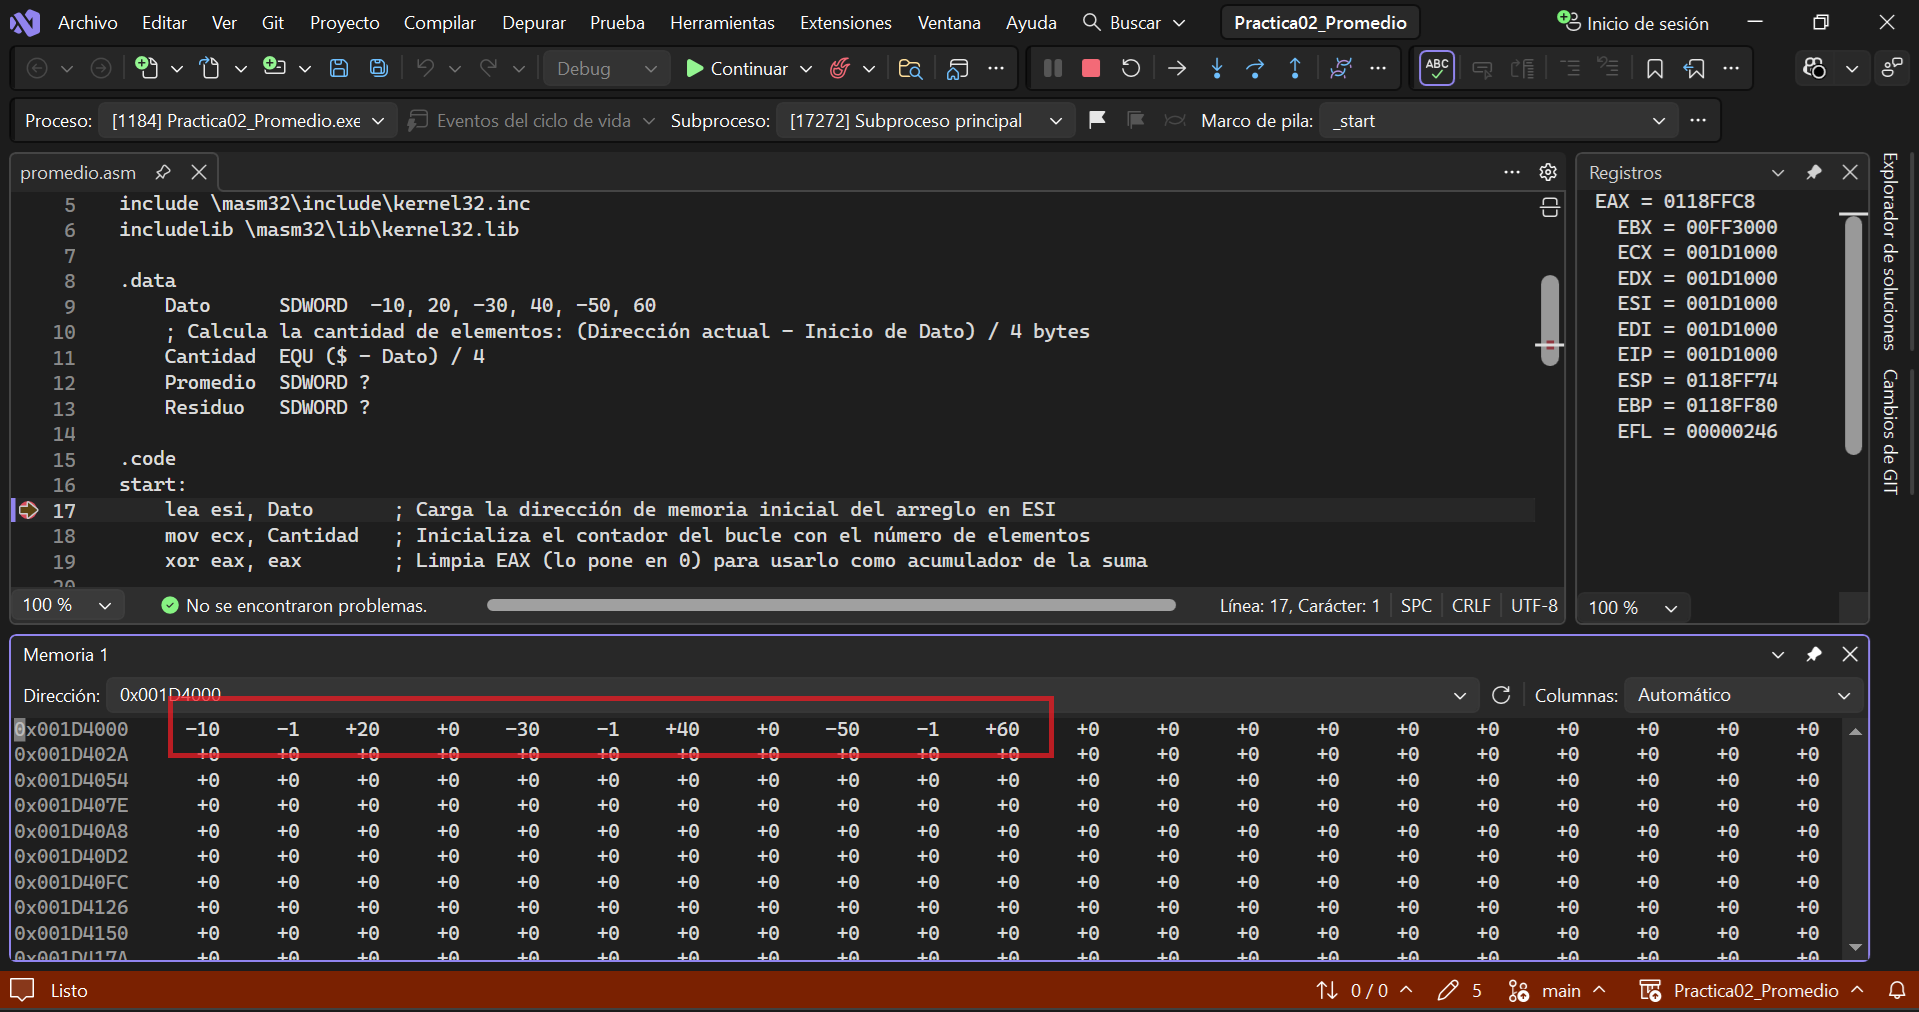
\includegraphics[width=1\textwidth]{registros_inicio.png}
    \caption{Estado inicial: ESI apunta a \texttt{Dato}, ECX = 6, EAX = 0}
    \label{fig:registros_inicio}
\end{figure}

\begin{table}[H]
    \centering
    \begin{tabular}{@{}cccc@{}}
        \toprule
        \textbf{Iteración} & \textbf{Elemento [ESI]} & \textbf{EAX (acumulador)} & \textbf{ECX restante} \\
        \midrule
        1 & $-10$ & $-10$ & 5 \\
        2 & $+20$ & $+10$ & 4 \\
        3 & $-30$ & $-20$ & 3 \\
        4 & $+40$ & $+20$ & 2 \\
        5 & $-50$ & $-30$ & 1 \\
        6 & $+60$ & $+30$ & 0 \\
        \bottomrule
    \end{tabular}
    \caption{Evolución del acumulador durante el ciclo \texttt{sumar}}
\end{table}

\begin{figure}[H]
    \centering
    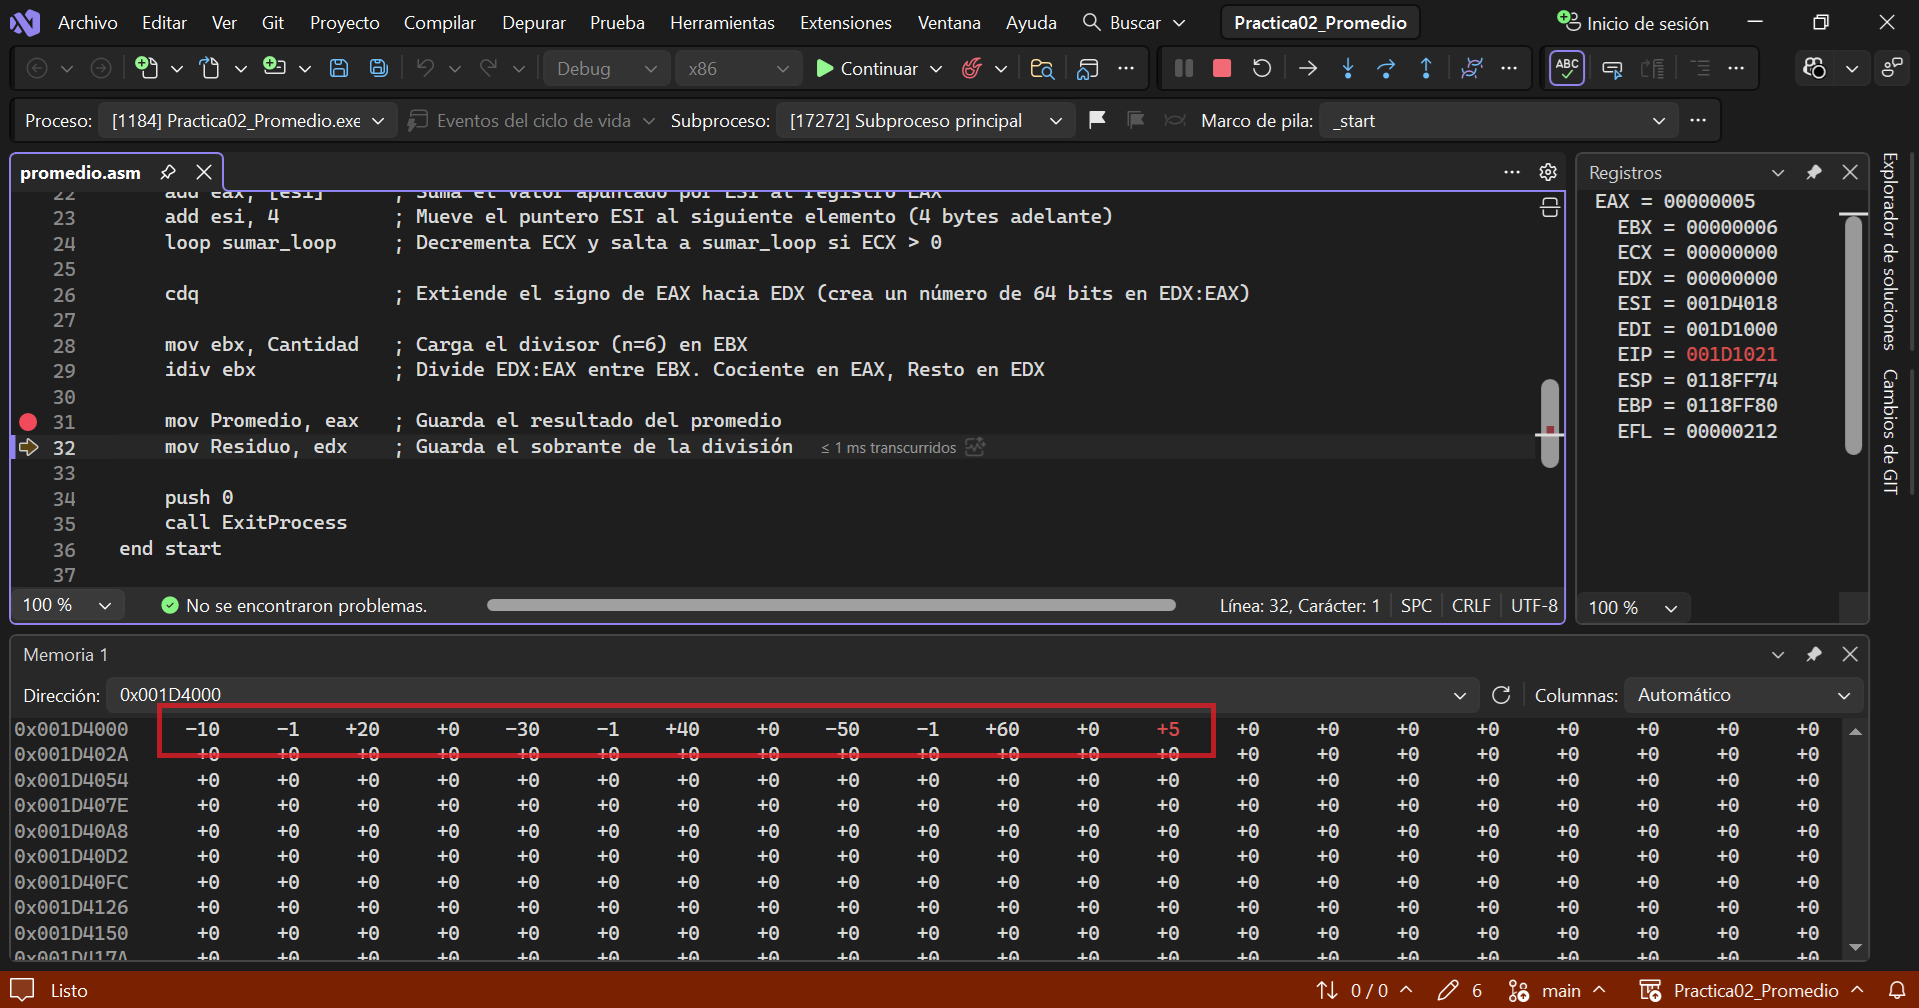
\includegraphics[width=1\textwidth]{memoria_resultado.png}
    \caption{Ventana de memoria: \texttt{Promedio = 0x05}, \texttt{Residuo = 0x00} escritos en \texttt{.data}}
    \label{fig:memoria_resultado}
\end{figure}

\begin{table}[H]
    \centering
    \begin{tabular}{@{}lcc@{}}
        \toprule
        \textbf{Variable} & \textbf{Registro origen} & \textbf{Valor almacenado} \\
        \midrule
        \texttt{Promedio} & \texttt{EAX} & $5$ \\
        \texttt{Residuo}  & \texttt{EDX} & $0$ \\
        \bottomrule
    \end{tabular}
    \caption{Valores escritos en \texttt{.data} al finalizar el programa}
\end{table}

% ============================================================
\section{Repositorio GitHub}

\url{https://github.com/7mo-ArquitecturaComputadoras/Practica02_Promedio}

% ============================================================
\section{Conclusiones}

\begin{itemize}
    \item El programa demuestra que \textbf{el procesador no distingue intrínsecamente entre suma y promedio}: el promedio no es más que una suma seguida de una división, y ambas operaciones se realizan directamente sobre registros.
    \item La instrucción \texttt{CDQ} es indispensable antes de \texttt{IDIV}: sin ella, \texttt{EDX} contendría valores arbitrarios y el resultado de la división sería incorrecto o provocaría una excepción, especialmente con sumas negativas.
    \item La directiva \texttt{EQU} con la expresión \texttt{(\$ - Dato) / 4} es un patrón idiomático en MASM para calcular el tamaño de un arreglo \textbf{en tiempo de ensamblado}, eliminando la posibilidad de errores al modificar la lista de datos.
    \item El uso de \texttt{LOOP} con \texttt{ECX} como contador ilustra cómo el hardware ofrece soporte nativo para estructuras de control como los ciclos \texttt{for} de los lenguajes de alto nivel.
    \item Esta práctica evidencia la cadena completa de operaciones que ejecuta un procesador cuando un lenguaje como Python o Java invoca \texttt{statistics.mean()}: en el fondo, el hardware realiza exactamente esta misma secuencia de sumas, extensión de signo y división con signo.
\end{itemize}

\end{document}
